\documentclass[../main.tex]{subfiles}
 
\begin{document}
	\section{Electromagnetic Induction}
	\begin{preamb}
		In the previous chapter we saw how a current can induce a magnetic field. In this chapter we will see the other side: how a magnetic field can induce a current.
	\end{preamb}

	\subsection{Fundamentals}
	\pdef{Electromagnetic Induction}{Electromagnetic induction is the process through which an induced electromotive force is produced in a conductor due to a changing magnetic field.}
	The two laws of electromagnetic induction are:
	\pdef{Faraday's Law}{Faraday's Law of electromagnetic induction states that the magnitude of the induced electromagnetic force is directly proportional to the rate of change of magnetic flux in the circuit. \[\varepsilon \propto \frac{\mathrm{d}\phi_B}{\mathrm{d}t}\]}
	Keep in mind it is the \textbf{change} in magnetic flux. If you put a coil of wire in a magnetic field and there is \textbf{no change}, then there is \textbf{no induced electromotive force}.
	\pdef{Lenz's Law}{Lenz's Law states that the direction of the induced electromotive force, and hence the induced current in a closed circuit, is always such that its magnetic effect opposes the motion or the change producing it.}
	\peqn{Faraday's Law for Solenoids}{\textit{(This is not in syllabus.)} Faraday's Law can be mathematically expressed as}{\varepsilon = -\frac{\mathrm{d}\phi_B}{\mathrm{d}t}}
	
	\subsection{AC Generators}
	The current flowing in the coil can be found using Fleming's right-hand rule.
	\begin{center}
		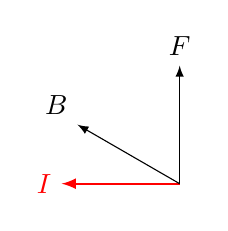
\begin{tikzpicture}
			\draw[-latex] (0,0) -- (0,1.5) node[anchor=south] {\(F\)};
			\draw[red, thick, -latex] (0,0) -- (-1.5,0) node[anchor=east] {\(\boxed{I}\)};
			\draw[-latex] (0,0) -- ({1.5*sin(300)}, {1.5*cos(300)}) node[anchor=south east] {\(B\)};
		\end{tikzpicture}
		\begin{framed}
			\textbf{R}ight-hand rule is for induced cu\textbf{r}rent.
		\end{framed}
	\end{center}
	
	Some important parts of the AC generator:
	\begin{itemize}
		\item \textbf{Armature:} the coil of wire mounted on the axle.
		\item \textbf{Slip Rings:} to ensure that the induced current in the coil is transferred to the external circuit.
	\end{itemize}

	The output voltage is a sinusoidal wave.
	\begin{center}
		\begin{tikzpicture}
%			\pgfplotsset{ticks=none}
			\begin{axis}[
				axis lines = middle,
				xlabel = \(t\)/\si{\second},
				ylabel = \(\varepsilon\)/\si{\volt},
				xtick ={
					0, 1.5708, 3.14159, 4.7123889, 6.28318
				},
				xticklabels={
					\(0\), \(\frac{T}{4}\), \(\frac{T}{2}\), \(\frac{3T}{4}\), \(T\)
				},
				ytick = {-1, 0, 1},
				yticklabels = {\(-\varepsilon_0\),\(0\),\(\varepsilon_0\)},
				ymax = 1.5,
				ymin = -1.5
			]
				\addplot [domain=0:6.3, samples=500] {sin(deg(x))};
				\draw [dashed, gray] (axis cs: 0,1) -- (axis cs: 6.3,1);
				\draw [dashed, gray] (axis cs: 0,-1) -- (axis cs: 6.3,-1);
				\draw [latex-latex] (axis cs: 4.7123889, -1) -- (axis cs: 4.7123889, 1) node[anchor=west, pos=0.75] {\(2\varepsilon_0\)};
				\draw [latex-latex] (axis cs: 1.5708, 0) -- (axis cs: 1.5708, 1) node[anchor=west, pos=0.5] {\(\varepsilon_0\)};
			\end{axis}
		\end{tikzpicture}
	\end{center}

	\subsection{Transformers}
	\pdef{Transformer}{A transformer is a device that can change a high alternating voltage (at low current) to a low alternative voltage (at high current), or vice versa.}
	\begin{itemize}
		\item \textbf{Primary coil:} connected to an alternating voltage \(V_P\);
		\item \textbf{Secondary coil:} output of the induced voltage \(V_S\);
		\item \textbf{Laminated soft iron core:} comprises of this sheets of soft iron. Because it is easily magnetised and demagnetised, this ensures better magnetic flux linkage between the two coils.
	\end{itemize}
	
	\begin{center}
		\begin{circuitikz}[]
			\begin{scope}
				\ctikzset{bipoles/cuteinductor/width/.initial=1.2}%default 0.6
				\ctikzset{bipoles/cuteinductor/coils/.initial=10}%default 5
				\draw (0, 0)  to [short, o-] +(1, 0)
				to [cute inductor, l=\(N_P\)]  +(0, 3)
				to [short, -o] +(-1, 0);
			\end{scope}
			%% vertical bare fore the core.  The middle is in y=1.5
			\draw[thick] (1.4, 0.5) -- (1.4, 2.5);
			\draw[thick] (1.6, 0.5) -- (1.6, 2.5);
			%% Secondary
			\draw(3, 0)  to [short, o-] +(-1, 0)
			to [cute inductor, l_=\(N_S\)]  +(0, 3) 
			to [short, -o] +(1, 0);
			\draw[latex-latex] (0,0.5) -- (0,2.5) node[pos=0.5, anchor=east] {\(V_P\)};
			\draw[latex-latex] (3,0.5) -- (3,2.5) node[pos=0.5, anchor=west] {\(V_S\)};
		\end{circuitikz}
	\end{center}

	\peqn{Turns Ratio}{The turns ratio of a transformer is calculated by}{\frac{N_P}{N_S} = \frac{V_P}{V_S}}
	The type of transformer can be determined from its turns ratio.
	\[\text{type of transformer} \begin{cases}
		\text{step-up} & N_S > N_P \\
		\text{step-down} & N_S < N_P
	\end{cases}\]
	
	\peqn{Conservation of Power}{Power is conserved in an ideal transformer,}{V_P I_P = V_S I_S}
	
	\subsection{Cathode Ray Oscilloscopes}
	\pdef{Oscilloscope}{Oscilloscopes are instruments used to observe how a voltage varies over time.}
	The graphic below shows an example of what a voltage varying over time might look like.
	\begin{center}
		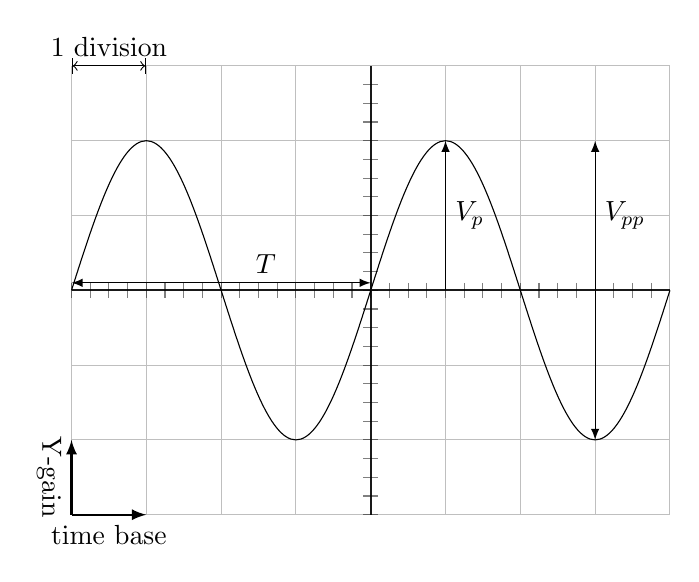
\begin{tikzpicture}[scale=0.95]
			\draw[|<->|] (-4,3) -- (-3,3) node[anchor=south, pos=0.5] {1 division};
			\draw[black, opacity=0.25] (-4,-3) grid (4,3);
			\draw[thick, gray!20!black] (0,-3) -- (0,3);
			\draw[thick, gray!20!black] (-4,0) -- (4,0);
			\draw[-latex, thick] (-4,-3) -- (-3,-3) node[anchor=north, pos=0.5]{time base};
			\draw[-latex, thick] (-4,-3) -- (-4,-2) node[anchor=north, pos=0.5, rotate=270]{Y-gain};
			\draw (-4,0) sin (-3,2) cos (-2,0) sin (-1,-2) cos (0,0) sin (1,2) cos (2,0) sin (3,-2) cos (4,0);
			\draw[-latex] (1,0) -- (1,2) node[anchor=west, pos=0.5] {\(V_p\)};
			\draw[latex-latex] (3,-2) -- (3,2) node[anchor=west, pos=0.75] {\(V_{pp}\)};
			\draw[latex-latex] (-4,0.1) -- (0,0.1) node[anchor=south, pos=0.65] {\(T\)};
			\foreach \y in {-3,-2,-1,0,1,2} \foreach \ys in {0,0.25,0.5,0.75} \draw[black, opacity = 0.5] (-0.1,{\y + \ys}) -- (0.1,{\y + \ys}); 
			\foreach \x in {-4,-3,-2,-1,0,1,2,3} \foreach \xs in {0,0.25,0.5,0.75} \draw[black, opacity = 0.5] ({\x + \xs},0.1) -- ({\x + \xs},-0.1); 
		\end{tikzpicture}
		\begin{framed}
			Keep in mind that \(V_p\), \textit{peak} voltage does \textit{not} necessarily refer to \(V_P\), \textit{primary} voltage. The \(p\) and \(P\) are different.
		\end{framed}
	\end{center}

	When reading an oscilloscope, always first identify the time base, in seconds/division [\si{\second/div}], and the Y-gain, in volts/division [\si{\volt/div}].
	
	\peqn{Complete Cycles}{The number of complete cycles of a voltage with frequency \(f_y\) shown in the oscilloscope with frequency of the time base \(f_x = \left(\text{time base}\right)^{-1}\) is given by the ratio}{\frac{f_y}{f_x}}
\end{document}